% from texdoc minted
\documentclass{elteikthesis}

\usepackage{t1enc}
\usepackage{ucs}
\usepackage[utf8x]{inputenc}
\usepackage[T1]{fontenc}
\usepackage[english,hungarian]{babel}
\selectlanguage{hungarian}

\usepackage{listings}
\usepackage{color}
\usepackage{verbatim}
\usepackage{minted}


\definecolor{mygray}{rgb}{0.4,0.4,0.4}
\definecolor{mygreen}{rgb}{0,0.8,0.6}
\definecolor{myorange}{rgb}{1.0,0.4,0}

\lstset {
	basicstyle=\footnotesize\sffamily\color{black},
	commentstyle=\color{mygray},
	frame=single,
	%%numbers=left,
	%%numbersep=5pt,
	%%numberstyle=\tiny\color{mygray},
	keywordstyle=\color{mygreen},
	showspaces=false,
	showstringspaces=false,
	stringstyle=\color{myorange},
	tabsize=2
}

\title{Interpoláció osztott rendszereken}
\author{Cselyuszka Alexandra}
\supervisor{Tejfel Máté}
\supervisorstitle{egyetemi tanár}
\period{Informatika Bsc}
\thesisyear{2015}
\department{Programozási Nyelvek és Fordítóprogramok Tanszék}
%%\additionaltext{ABCDEF GHIJKLM NOPQRSTUV WXYZ}

\begin{document}

\frontmatter

	\maketitle

\mainmatter

\tableofcontents
	
\chapter{Bevezetés} 

\textit{
"A gyakorlatban sokszor felmerül olyan probléma, hogy egy nagyon költségesen kiszámítható függvénnyel kellene egy megadott intervallumon dolgoznunk. Ekkor például azt tehetjük, hogy néhány pontban kiszámítjuk a függvény értékét, majd keresünk olyan egyszerűbben számítható függvényt, amelyik illeszkedik az adott pontokra." }\cite{numanalbev}
\newline
\newline
A szakdolgozatom célja ezekre a problémákra megoldást adni elosztott környezetben. 
\section{Feladat elemzése}
Adott ponthalmazokból kívánunk egy közelítő polinomot becsülni. Ezeket különböző interpolációs technikával meg tudjuk adni, ki tudjuk számolni. Több interpolációs technika létezik, melyekből könnyen meg tudunk adni akár több polinomot is egy adott ponthalmazhoz.\newline
Ezekkel a számításokkal előfordulhat, hogy lassan futnak, főleg ha több interpolációt kívánunk egyszerre számolni.
Ebben az esetben optimálisabb több gépen számolni a különböző ponthalmazokat.
\newline\newline
Ebben a feladatban egy speciális megvalósítása lesz ennek a számításnak. 
\newline
A grafikus része egy weboldal, melyen szerkeszthetjük a ponthalmazokat. A számítás részét egy szerver végzi amely figyeli a felcsatlakozó gépeket. Amikor kap egy számítandó adathalmazt, akkor több gép segítségével kiszámítja az eredményt. Ha minden részfeladat végzett, akkor vissza küldi a weboldalra, ahol az eredmények megtekinthetőek grafikus formában.
\newline\newline
\section{Feladat megvalósítása}
A \textbf{grafikus felület}  egy weboldal, mely JavaScript-ben és HTML-ben van megvalósítva.
 A felületen egy listát tekinthetünk meg, ahova több ponthalmazt is felvehetünk. \newline  Mentés hatására az értékek a háttérben eltárolódnak. A ponthalmazok közül választhatunk egyet, amely betöltődik felületre.\newline A szerkesztő felület egy táblázatból és egy grafikonból áll, emellett még a különböző speciális számításra vonatkozó tulajdonságok (interpoláció típusa) valamint a grafikonon való megjelenítéshez tartozó tulajdonságok (polinom pontosság, megtekintendő intervallum) is szerkeszthetőek. \newline Ha befejeztük a halmazok szerkesztését elküldhetjük a számítani kívánt értékeket a szerver felé.
 \newline\newline
A \textbf{szerver} feladata hogy figyelje a felületről érkező adatokat. Ha az adathalmaz megérkezett, akkor a szerver kibontja az adatokat egy JSON-ból, és elindítja az elosztást. \newline
Az elosztáshoz a szerveren el kell indítani egy figyelő folyamatot amelyre lehetősége van egy külső gépnek felcsatlakozni. Amikor a szerveren indul egy számolás a felcsatlakozott gépeket lekérdezi, majd a feladatokat szétosztja.\newline
A szerver megvalósítása és a gépekre való szétosztás Erlang-ban lett megvalósítva. A JSON feldolgozásához mochi-json lett alkalmazva. A feldolgozás után az adathalmazon végig megyünk és azok alapján felparaméterezzük, és meghívjuk a számítást végző függvényt.\newline
A számításhoz használt maximális gépek száma paraméterként megadható, de a tényleges számítást csak annyi gépen tudjuk maximálisan végezni ahány gép felcsatlakozott a számításhoz.
\newline\newline
A \textbf{számítás} megvalósítása C++ nyelven történt. A paraméterek alapján a Lagrange -féle, Newton -féle, Hermite -féle interpolációs technikák közül eldönti melyik esetet használja.\newline
A programban kellett implemetálni egy egyszerű polinom szorzás és összeadást, valamint az interpolációkhoz szükséges függvényeket. Lagrange számítás a polinom műveletek és a képlet felhasználásával ciklusokkal valósul meg. Newton és Hermite esetén a kapott adatokból először a kezdő mátrixot kell legenerálni, majd kiszámítani. \newline
Abban az esetben ha Newton vagy Lagrange polinomot számolunk nem vesszük figyelembe a derivált pontokat, viszont figyelembe vesszük ha inverz számítást kívánunk végezni. 


\chapter{Felhasználói dokumentáció}
\begin{comment}
A Felhasználói dokumentáció tartalmazza
- a megoldott probléma rövid megfogalmazását,
- a felhasznált módszerek rövid leírását,
- a program használatához szükséges összes információt

Magába foglalja a telepítési- (vagy üzemeltetési-) és a végfelhasználói leírást. Ezek
meghatározott célközönséghez szólnak, könnyen és gyorsan kell, hogy eligazítsák a
felhasználót a program használatában!

\end{comment}
\section{Bevezetés}
%% A feladat rövid ismertetése (mire való a szoftver)
%% Célközönség (kik, mikor, mire használhatják a programot)
\section{Telepítési útmutató}
\subsection{Rendszer követelmények}
%% A rendszer használatához szükséges minimális, illetve optimális HW/SW környezet
\subsection{Segédprogramok telepítése}
%% Első üzembe helyezés leírása – ha van ilyen –, a program indítása (kivéve, ha nem egy
%%önálló alkalmazásról, hanem egy meglévő rendszer új komponenséről van szó). Itt
%%ellenőrizzük, hogy a telepítési útmutató megfelel-e a valóságos telepítési folyamatnak.
\subsection{Szerver és segédgépek üzembe helyezése}
\subsection{Használati útmutató}
\subsubsection{Weboldal}
\subsubsection{Szerver}
%% Általános felhasználói tájékoztató (például a szokásostól eltérő képernyő-, billentyű-,
%%illetve egérkezelés leírása, teendők hibaüzenetek esetén stb.).
%% A rendszer funkcióinak ismertetése. A feladat jellegéből fakadóan célszerű lehet ezt
%%folyamatszerűen, képernyőképekkel alátámasztva bemutatni. A funkciókat ajánlatos a
%%felhasználói szintek szerint csoportosítani. Itt vegyük figyelembe, hogy a leírás a
%%fejlesztői dokumentációban meghatározott részfeladathoz illeszkedik-e, az ott
%% meghatározott funkciókat/használati eseteket írja-e le?
%% A rendszer futás közbeni üzenetei (hibaüzenetek, figyelmeztető üzenetek, felszólító üze-
%%netek stb.) és azok magyarázata – az esetleges üzemeltetési teendőkkel együtt. Itt vegyük
%%figyelembe, hogy tartalmaz-e biztonsági, illetve hibaelhárítási előírásokat?
%% Egyéb, a szoftver használatához szükséges információk.


\chapter{Fejlesztői dokumentáció}
\begin{comment}
A Fejlesztői dokumentáció tartalmazza
- a probléma részletes specifikációját,
- a felhasznált módszerek részletes leírását, a használt fogalmak definícióját,
- a program logikai és fizikai szerkezetének leírását (adatszerkezetek, adatbázisok,
modulfelbontás),
- a tesztelési tervet és a tesztelés eredményeit.
\end{comment}

%% ----------------------------------------------{Megoldási terv}
\section{Megoldási terv}
A program működésileg 2 részre bontható: weboldalra(kliens) és a szerverre.
A weboldalon össze állított adatokat küldjük fel a szerverre, a szerver a megkapott adatok alapján számol. \newline
\subsection{Weboldal}
	A kliens megvalósításához az alábbi technológiák merültek fel : C++/Qt, C\#, JS/HTML. Végül JavaScript-ben lett megvalósítva, első sorban a grafikon kirajzoló Flot miatt, de a szerver kommunikáció egyszerűsége is döntő ok volt amellett, hogy egy weboldal bármely gépen egyszerűen megnyitható, kezelhető.\newline
	Egy oldalból áll melyen a felhasználó szerkesztheti az adatokat. Azért nem lettek a részek külön oldalakon megvalósítva, mert az egyik oldalról az adatok átvitele egy másik oldalra nem annyira egyszerű, viszont nincs is olyan komplex az oldal, hogy szükséges legyen több aloldalra szétbontani. 
	Az oldal megjelenés felépítése megtekinthető \ref{fig:weblap_vazlat}-es képen.
	\begin{figure}[h]
	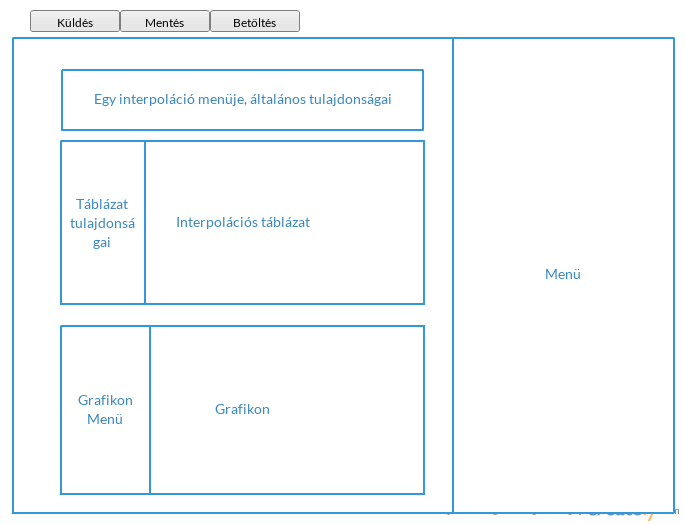
\includegraphics[width=14cm]{pics/weblap_vazlat}
	\centering
	\caption{Weboldal vázlata\label{fig:weblap_vazlat}}
	\end{figure}
	A weboldalon meg kell valósítani a pontok dinamikus kirajzolását, és a táblázatos formában történő megjelenítést és szerkeszthetőséget. Mivel több interpolációt küldünk fel a szervernek ezért a weboldalon több szerkesztésére is lehetőséget kell adni. \newline 
	Több szerkesztésének megvalósításához kell egy menü rendszer, amelyben eltárolódnak az adatok, és képesek betöltődni.\newline
	Az oldalon input-okat használunk még, és a dinamikus táblázat is JavaScript-ből van legenerálva. A táblázatokban sorok beszúrására teljes táblázat törlésre is lehetőséget kell adni. 
	A táblázatokban inputok vannak az egyes cellákban melyben egyszerű értékek, vagy akár komplexebb Objektumok is találhatóak. A bonyolultabb objektumokat json string-ben tároljuk ezekben az inputokban. \newline
	A menü listájában új adathalmazokat hozhat létre, a régieket szerkesztheti.
	Amikor a felhasználó pontokat, megjelenítést frissít a legtöbb esetben az oldal már a háttérben menti az adatokat a listába. Amikor egy másik interpolációt választunk ki, akkor az betöltődik a táblázatba, és a grafikonba. A módosításoknál az értékei az ő oszlopában fognak törlődni.
	Ha a felhasználó végzett egy gombra nyomással a program legenerálja a szükséges objektumot. \newline
	A felület sok gombot tartalmaz, melyek hatására frissíthetőek az adatok. Amikor frissítünk egy részt, általában mentődnek az értékek egy inputba JSON formában.\newline
	A felület manuális teszteléssel lett kipróbálva, automatizált tesztesetek nem lesznek.
  	\subsubsection{Grafikon kirajzoló - Flot}

	\begin{figure}[h]
	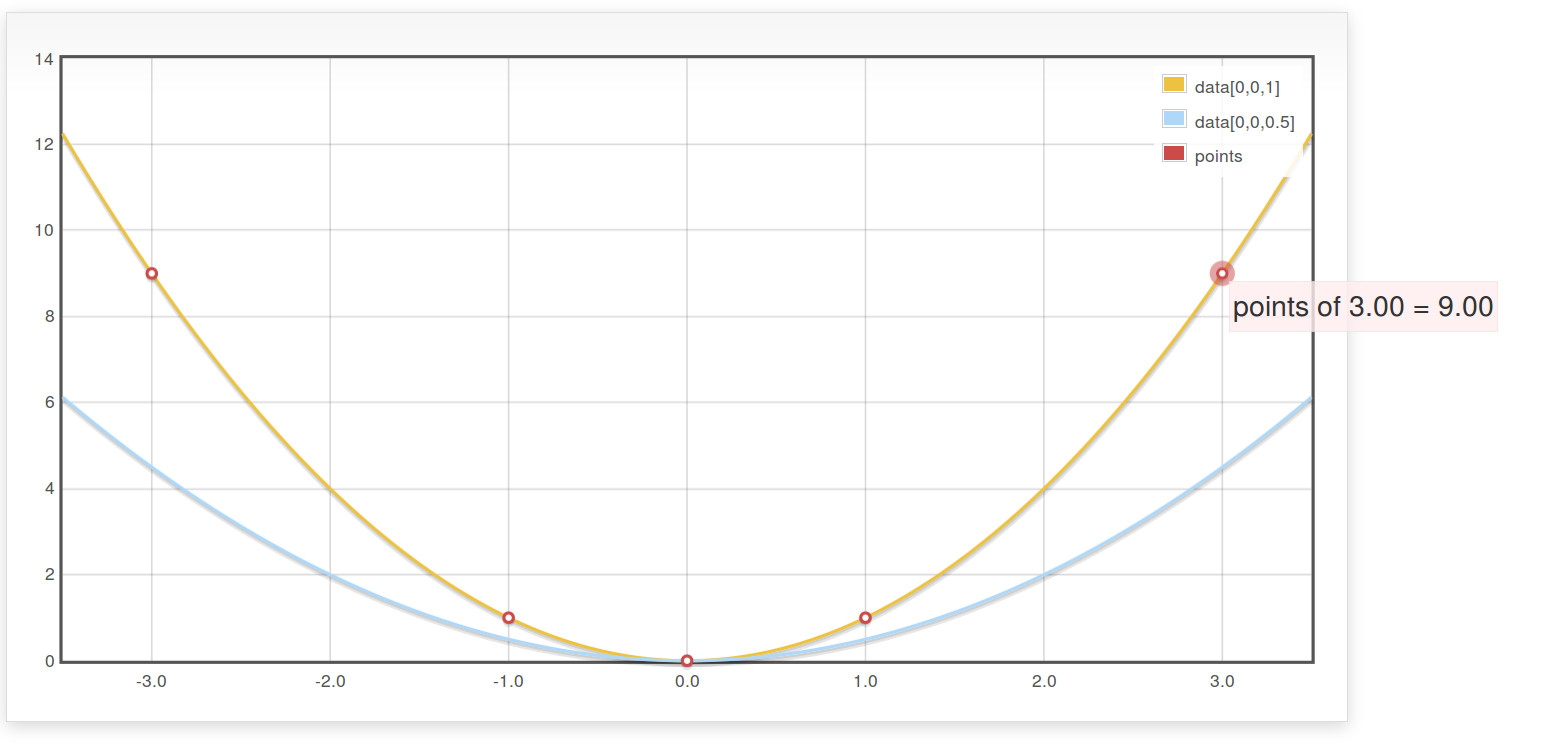
\includegraphics[width=13cm]{pics/plot}
	\centering
	\caption{Grafikon kirajzoló\label{fig:plot}}

	\end{figure}
		A Grafikon megjelenítéséhez a flot-ot használom. Ez egy jQuery-s könyvtár, melyben egyszerűen és látványosan lehet grafikonokat kirajzolni. A forrás a "WebPage/source/flot-8.0.2" mappában érhető el.
		HTML fájlban egy egyszerű div-ként jelenik meg, melyet aztán a JavaScript tölt meg tartalommal.
				\begin{minted}{html}
	<div id=\"resultplot\" class=\"demo-placeholder\"></div>
			\end{minted}
		A JavaScript-ben hivatkozhatunk erre a div-re, majd az adatok és a típusok segítségével alábbi módon hivatkozhatjuk meg: 
		\begin{minted}{javascript}
	    var placeholder = $("#resultplot");
	    var plot = $.plot(placeholder, flot_data, type);
		\end{minted}
		A paraméterezése a grafikon kirajzolónak az alábbi: 
		\begin{description}
			\item[placeholder] \hfill \\ 
	 			DIV hivatkozása
	 		 \item[type] \hfill \\ 
	 			Megjelenítendő grafikon típusa
	 			\newline
	 			A flot sok lehetőséget nyújt a típusok kiválasztására, és ezekre való példákból megalkottam a saját típusomat mely a következőket tartalmazza egy Object\{\}-ben:
		 		
		 		\begin{verbatim}
		 			series: { line: { show: true } } 
		 		\end{verbatim}
				Beállítjuk hogy a vonalakat jelenítse meg. Ekkor a pontokat is megjeleníti, a többi beállítás függvényében.
		 		
		 		\begin{verbatim}
					xaxis: { zoomRange: [0.1, 1], panRange: [-1000, 1000] }
					yaxis: { zoomRange: [0.1, 100], panRange: [-1000, 1000] }
		 		\end{verbatim} 
		 		X és Y kordinátákon nagyítás és mozgatási beállítások interaktívvá állítása
			 	\begin{verbatim}
			 		grid: { hoverable: true, clickable: true }
			 	\end{verbatim} 
			 	Ezeket a tulajdonságokat használjuk arra hogy felvegyünk új pontokat.
			 	Emellett ha ráviszem az egeret az egyik pontra, megmutatja a pont koordinátáját, és értékeit, és hogy melyik ponthalmazon van.
			 	\begin{verbatim}
			 		zoom: { interactive: true}, pan: { interactive: true }
			 	\end{verbatim} 
			 	Nagyítás és kattintással mozgatás engedélyezése. \newline
				Ennek a beépítésével is foglalkoztam, de a kattintás sajnos nem egyeztethető könnyen össze a pont figyeléssel, valamint a beépítés után lassú lett, és akadozott a felület, így végül az interaktivítását külső komponensekkel(inputokkal) oldottam meg.

	 		\item[flot\_data] \hfill \\ 
	 		A tényleges adathalmazokat tartalmazó tömb, melyben az egyes adatokról egyéni információkat is tartalmazza.\newline
	 		\begin{description}
				\item[data] \hfill \\ 
				Pontok halmaza, melyeket megjelenítünk\newline
				[x, y] pontokból álló tömb\newline
				Polinom esetén is ezt használjuk, ezért a polinom behelyettesített értékeit adjuk itt meg. Amikor az egérrel felé megyünk ezeket a pontokat fogja megjeleníteni.
				\item[label] \hfill \\ 
				Adathalmaz elnevezése, ezt láthatjuk amikor az egérrel a pont felé visszük az egeret, valamint a színek-elnevezések össze párosításánál is segít.
				\item[points] \hfill \\ 
				Ha pontokat szeretnénk megjeleníteni, akkor ezt a kapcsolót kell alkalmazni.
				\item[lines] \hfill \\ 
				Ha a pontokból alkotott vonalat szeretnénk látni, akkor ezt a kapcsolót kell alkalmazni. Ezt használjuk a polinom megjelenítéséhez.
			\end{description}
	 		\begin{minted}{javascript}
		var example_datas = [{
			data: d4,
			label: "neved4",
			lines: { show: true }
		}, {
		    data: d3,
			label: "neved43"
		    points: { show: true }
		}];
			\end{minted}
		\end{description}

\subsection{Elosztott rendszer}
	Az elosztott rendszer megvalósításához az alábbi technológiák merültek fel: C++/PVM, Erlang.
	Miután a JavaScript mellett döntöttem a grafikus felületen, ezután optimálisabbnak tűnt egy hasonlóan gyengén típusos nyelvnek a használata. Az erlang elég jól támogatja párhuzamosítást és a szerver kommunikációt is, és bár az algoritmusok implementálása nehézkesebb lett volna, de C++-ban megvalósított függvények beépítése miatt ez a probléma megoldódott.

	\subsubsection{Http szerver}
	A http szerver gyakolratilag 2 példából lett megvalósítva:
	"simpleServer leírása TODO"
	\subsubsection{Node figyelő}
	"pingPong TODO: pidWatcher mit csinál"
	\subsubsection{Struktúra kezelő}
	"structHandler"
	\subsubsection{Elosztás}
	"nodeHandler"

\subsection{Számítás}
	A számítás megvalósításánál felmerült hogy Erlang-ban legyen, de mivel a számítást ciklusokkal érdemes megvalósítani, ezért egyszerűbb volt egy nem funkcionális nyelvben implementálni azokat.
	A C++-os függvényeket nem volt bonyolult felhasználni Erlang-os modulként. 

\subsection{Kommunikáció}
	Amikor a szervert létrehozzuk akkor inicializálunk két proceszt. Az egyik a kliens felől várakozik kérésre, a másik a nodeok felől. Amikor egy node fel kíván csatlakozni küld egy kérést a regisztációra. Ha sikeres volt akkor a szerver ezt jelzi neki, és felkerül a listára. \newline
	A weboldalon egy gomb hatására megy egy kérés a szerver felé. A szerver jó esetben fogadja a kérést. Ha nem sikerült kapcsolatba lépnie a szerverrel, akkor jelzi a felhasználónak hogy a kapcsolódás során hiba lépett fel. \newline
	Ha fogadta a kérést, akkor megpróbálja feldolgozni az adatokat. Ha sikeresen feldolgozta az adatokat, abban az esetben elindul a szétosztás. \newline
	A szétosztás során a felcsatlakozott gépeken létre jönnek a processzek, majd kapnak egy adathalmazt mellyel számolniuk kell. Ha végeztek, az eredményt vissza küldik a szülő processznek. A szülő processz, ha megkapott minden értéket, azt vissza küldi a weboldalnak.
	\newline
	A weboldal sikeres válasz után betölti az eredményeket. 
	\begin{figure}[h]
		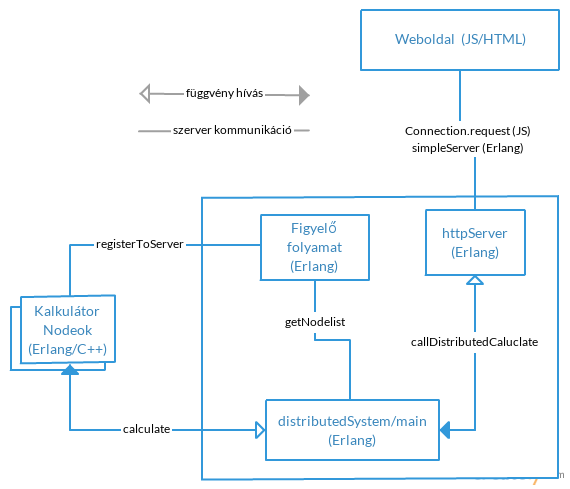
\includegraphics[width=13cm]{pics/kommunikacio1}
	\centering
	\caption{Kommunikáció\label{fig:kommunikacio1}}
	\end{figure}

%% ----------------------------------------------{Weboldal}
\section{Weboldal megvalósítása}
\subsection{Felépítés}
	A weboldal forráskódja a /webpage mappában helyezkedik el. 
	A fájlszerkezet az alábbi:
	\begin{description}
		\item[webpage.js :] \hfill \\  
		Globális változók inicializálása és pár alapbeállítás lefuttatása
		
		\item[webpage.html :]  \hfill \\ 
		Weboldal megjelenítése, fájlok betöltése
		
		\item[init] \hfill \\ 
		Inicializáló függvények hívásai és események
		\begin{description}
			\item[menulist.js : ] \hfill \\ 
				Interpolációk listájának inicializálója
		  	\item[plot.js : ] \hfill \\ 
		  		Interpolációs grafikon inicializálása
			\item[table.js : ] \hfill \\ 
				Interpolációs táblázat inicializálása
		 	\item[events.js : ] \hfill \\ 
		 		Gombra kattintások eseményei
		\end{description}

		\item[model] \hfill \\ 
		Objektumok, melyeket az inicializáló lépésben hívunk, és azok segédletei
		\begin{description}
		 	\item[base.js : ] \hfill \\
		 		Globális függvények \newline
		 		Base.get, Base.erlangJSON, Base.forEach
		 	\item[base\_table.js : ] \hfill \\
		 		Általános táblázat generáló függvény
		 	\item[connection.js : ] \hfill \\
		 		Szerver kapcsolat meghívására szolgáló függvény \newline
		 		Connection.request
		 	\item[plot\_types.js : ] \hfill \\
		 		A grafikon kirajzoló típus objektumai
		 	\item[polinome.js : ] \hfill \\  
		 		Polinom kirajzolását segítő függvények \newline
		 		makePolinome található benne és egyéb segédfüggvények
		 	\item[web\_page\_debug.js : ] \hfill \\ 
		 		A Weboldalon történő logolást segítő objektum \newline
		 		Jelenleg sehol nem használjuk már, de a megvalósítás során fontos szerepe volt a hibajavításban
		\end{description}
		\item[model/interpolation] \hfill \\
		Az oldal 3 fő részegységének függvényei
			\begin{description}
			\item[menulist.js : ] 
				Interpolációk lista megvalósítása \newline
				function interpolationMenulist (aConfig) Objektum fájlja
		  	\item[plot.js : ] \hfill \\ 
		  		Interpolációs grafikon megvalósítása \newline
				function interpolationPlot(aConfig) Objektum fájlja
			\item[table.js : ] \hfill \\
				Interpolációs táblázat megvalósítása \newline
				function interpolationTable(aConfig) Objektum fájlja
			\end{description}
	\end{description}
\subsection{Fontosabb objektumok és függvények}
	\hfill
	Az objetumokat legtöbb esetben egy függvény generálja, melyben \"that.\"-al jelöltek azok, melyeket a visszatérés után felhasználunk az eseménykezelésekhez.
	\begin{description}
		\item[makePolinome(inPolinome, plotFor)] \hfill \\ 
			Polinom pontjainak legenerálására szolgáló függvény, a grafikon kirajzolónak megfelelő típusban
			\begin{description}
				\item[inPolinome] polinom
				\item[plotFor] polinom intervalluma és pontossága
			\end{description}
		\item[Connection.request(aConfig)] \hfill \\ 
			Elküldi a szervernek az értékeket
			\begin{description}
				\item[aConfig.params] a kommunikációban a paraméter amelyet átküldünk a szervernek
				\item[aConfig.callback] sikeres visszatérés esetén lefutó függvény
			\end{description}
		\item[basicTable (aConfig)]
			\hfill \\ 
			Egy alap tábla objektum. Ennek segítségével lehet létrehozni az interpolációs táblázatot és a menülistát(interpoláció választó)
			\begin{description}
			\item[that.addNewCellToRow(rowIndex, textValue, inputAttributes)] 
				\hfill \\  Ad egy új cellát a sorhoz
			\item[that.addNewRowToTable(data)]
				\hfill \\ Ad egy új sort a táblázathoz
			\item[that.addNewColumnToTable(data)]
				\hfill \\ Ad egy új oszlopot a táblázathoz
			\item[that.newTable()] 
				\hfill \\ Új tábla létrehozása
			\item[that.setCellForm((i , j, attributes))] 
				\hfill \\ Egy adott cella megformázás beállítása
			\item[that.getNumOfCols()] 
			 	\hfill \\ Vissza adja az oszlopok számát
			\item[that.getNumOfRows()]
				\hfill \\ Vissza adja a sorok számát
			\item[that.getRow(i)]
				\hfill \\ Vissza adja a sort az index alapján. 
				Ha nincs olyan indexű akkor null
			\item[that.getInputTag(i, j)]
				\hfill \\ Vissza tér a tábla input elemével
			\item[that.getValue(i, j)]
				\hfill \\ Egy adott cella érték lekérdezése
			\item[that.findValue(column, value)] 
				\hfill \\ Megkeresi melyik sorban van egy adott értéket
			\item[that.setValue(i, j, value, form)]
				\hfill \\ Beállít egy adott értéket egy cellának
			\item[that.deleteTable()]
				\hfill \\ Teljesen törli a táblázatot
			\item[that.remove(row)]
				\hfill \\ Kivesz egy sort a táblázatból
			\item[addNewRowTagToTable ()]
				\hfill \\ Ad egy új sort a táblázathoz
			\item[addCellToRow(index)]
				\hfill \\ Ad  egy cellát a sorhoz
			\item[setAttributes(object, attributes)]
				\hfill \\ Beállítja egy objektum tulajdonságait
			\item[makeTextInput (value,  attributes)]
				\hfill \\  TextInput hozzáadása a sorhoz
			\end{description}
		\item[interpolationMenulist (aConfig)] 
			\hfill \\ 
			Az interpolációs menü függvénye. Itt tarjuk számon az aktuálisan betöltött adathalmazt.
			\begin{description}
			\item[that.newItem()] 
			\hfill \\ Új Lista elem
			\item[that.getDataArray(server)] 
			\hfill \\ Vissza adja az adathalmazt, tömb formában. Ebben a formában küldjük fel a szervernek.
			\item[that.getDataObject()] 
			\hfill \\ Vissza adja az adathalmazt, egy objektum formájában. Az Objektum értékeinek kulcsa, az interpolációk id-ja.
			\item[that.saveItemSettings()] 
			\hfill \\ Elmenti az adatokat az aktuálisan kijelölt sorba.
			\item[that.loadItemSettings(index)]
			\hfill \\ Feldogozza az adatsort a táblából, és betölti az adatokat a táblába.
			\item[that.loadAll(savedObject, resultObject)] 
			\hfill \\Betölti az összes Interpolációt az adott adathalmazból
			\item[newMenulist()] 
			\hfill \\
			Új menülista: régi menü kitörlése, és egy új generálása
			\hfill \\ 
			\end{description}
		\item[interpolationPlot (aConfig)]
			\hfill \\ Grafikon megjelenítése: "Flot" segítségével létrehoztam az alábbi Objektumot. Ebben valósítottam meg a kirajzolást, és annak tulajdonságait.
			\begin{description}
			\item[that.refresh(points, polynomials)]
			\hfill \\ Pontok és a polinomok alapján frissíti a grafikont
			\item[that.getPlotSettings]
			\hfill \\ Visszatér a grafikon megjelenítési tulajdonságokkal. Ennek segítségével mentünk.
			\item[that.setPlotSettings]
			\hfill \\ Betölti a grafikon megjelenítési tulajdonságokat.
			\item[generateData(senderData, polynomial)]
			\hfill \\ Legenerálja a grafikon azon bemenő paraméterét, amely a megjelenítendő adatokat állítja,

			\item[generateType()]
			\hfill \\ Legenerálja a grafikon azon bemenő paraméterét, amely a grafikon megjelenítését állítja
			\item[setDefaultSettings()]
			\hfill \\ Legenerálja a grafikon azon bemenő paraméterét, amely a grafikon megjelenítését állítja
			\item[generatePointSet(tableArray, derivNum)]
			\hfill \\ Legenerálja az adott pontokat, az interpolációs táblázatból
			\end{description}

		\item[interpolationTable (aConfig)]
			\hfill \\ 
				Az interpolációs Táblázat logikája, és generálása. Ebben a táblázatban tekinthetjük meg a pontokat.
			\begin{description}
			\item[that.addPoint(x, y, dn)] 
			\hfill \\ Hozzá adja a pontot a táblázathoz. Ha létezik ezen az X-en pont akkor frissíti.
			\item[that.setPoints(tableArray)] 
			\hfill \\ Feltölti a táblázatot egy adott tömb értékeivel
			\item[that.setData(data)] 
			\hfill \\ Feltölti az adatokkal a táblát
			\item[that.getData()] 
			\hfill \\ Vissza adja a táblázatban szereplő adatok
			\item[that.getPoints()] 
			\hfill \\ Vissza adja a táblázatban szereplő pontokat
			\end{description}
	\end{description}



%% ----------------------------------------------{Elosztott rendszer}
\section{Elosztott rendszer  megvalósítása}
Elosztott rendszer Erlang-ban lett megvalósítva. Az elosztást interpolációnként végezzük, vagyis annyi node-ot hozunk létre amennyi interpolációt kívánunk egyszerre kiszámítani. \newline
A szerver figyel egy portot hogy érkezett-e rá adat. Ha érkezett adat az adott portra, azt kibontja, és elvégzi a szükséges műveleteket. A JSON-t kibontja, és feldolgozza. Kinyer belőle egy listát mely az interpolálni kívánt pontokat és tulajdonságokat tartalmazza. \newline
Tudjuk pontosan hány eleme van a listának, és annyi processzt hozunk létre. Ha vannak felcsatlakozva Node-ok akkor a processzt az adott node-on is meg tudja hívni.
Ha létrehozta a processzeket lista elemein végig megy, és azokat szétküldi a processzeknek, majd megvárja míg az összes végig ér, és vissza térve megkapja az eredményt.
\subsection{Web-szerver kommunikáció}
	A webszerver kommunikációhoz a fájlok a simpleServer.erl fájlban találhatóak meg. Az ebben találhat függvényeket a main-ben hívjuk meg. Amikor inicializáljuk a szervert.
	\begin{description}
	\item[simpleServer:start(Port, WatcherNode)] 
		\hfill \\
		Elindítja a szervert, az adott porton. \newline
		Ezt a függvényt a main-ben hívjuk, meg ahol már megkapja a node-figyelő pid-jét és az alapértelmezett port-ot 
	\item[simpleServer:response(Str, WatcherNode)] \hfill \\ 
		Miután érkezik egy kérés a szervernek ebben a függvényben kezeljük le. Innen indul ki minden folyamat ami a számítást végzi. \newline 
		Az alábbi sorrendben hívódnak meg a függvények: \newline
		getDecodeData, convertData, callMain, convertToSend
	\item[simpleServer:getDecodeData(\_)] \hfill \\ 
		Vissza tér a szervernek küldött paraméterrel
	\item[simpleServer:convertData(ResponseParams)] \hfill \\ 
		Létrehozza a kapott adatból az Erlang struktúrát
	\item[simpleServer:callMain(RespJson, WatcherNode)] \hfill \\ 
		Amikor az adatokat feldolgoztuk és minden rendben ment, elindítjuk a main függvényét, ezen függvény segítségével.
	\item[simpleServer:convertToSend(Object)] \hfill \\ 
		Amikor a számítás véget ért, létrehozzunk a visszaküldéshez szükséges adatstruktúrát, majd elküldjük a szervernek.
	\end{description}
\subsection{Web-szerver Adat feldolgozás}
	Az adatot JSON-ben kapja a szerver. Az adathalmaz kibontásához MonchiJSON lett alkalmazva. 
	A segédfüggvények és konvertálók a "distributedSystem/struch\_handler.erl" fájlban lettek megvalósítva.\newline
	Elsősorban a megkapott speciális adathalmaz kibontására használtak az itt lévő függvények, de egyéb segédfüggvények is megtalálhatóak ebben a fájlban, amelyek a konvertálással kapcsolatosak.

	\subsubsection{\underline{
		MochiJSON kibontásához használt segédfüggvények:
	}}
	\begin{description}
		\item[struct\_handler:getElementByKeyList(KeyList, DataSetElement)] \hfill \\ 
		Vissza tér egy értékkel, amely az adott kulcson van, ha egy elemű a kulcs lista. Több elem esetén a kulcsokban lévő értékeket nézi, és vissza adja a legbelső kulcson lévő elemet.

		\item[struct\_handler:getElementByKey()] \hfill \\ 
		Vissza tér egy objektumban az adott kulcson lévő értékkel
	\end{description}
	\subsubsection{\underline{Adat Struktúra az interpoláció meghívásához}}
	\begin{description}

		\item[struct\_handler:getDataByJson(JsonSting)] \hfill \\
		A mochi-json dekódoló meghívása, vissza tér egy Erlang struktúrával.
		
		\item[struct\_handler:getDataSet(Data)]\hfill \\ 
		Vissza tér az adatok halmazával. Ebből a halmazon, vagyis listán kell végig menni, és szétosztani az elemeit. 
		
		\item[struct\_handler:getPoints] \hfill \\
		Pontok vissza nyerése egy speciális módon, melyet a "calulator" fel tud használni

				\begin{minted}{erlang}
EmptyStruct =  [{x, []}, {y, []}]
		\end{minted}


		\item[struct\_handler:<Számítási paraméterek>] \hfill \\ 
		getInverse(DataSetElement) - inverz-e \newline
		getType(DataSetElement) mi a típusa? \newline
		getId(DataSetElement) egyedi azonosítója \newline
		getPoints(DataSetElement) pontok struktúrája
	\end{description}
	\subsubsection{\underline{Az eredmény vissza nyeréséhez az alábbi segédfüggvényeket kellett használni:}}
	\begin{description}
	
		\item[struct\_handler:convertToMochi(Object)] \hfill \\ 
		A Mochi struktúra annyira nem egyértelmű elemekből áll. Speciálisan kell felépíteni az eredményt. Ez a függvény megkap egy Erlang listát és átkonvertálja MochiJSON-nek megfelelő struktúrává, majd
		
		\item[struct\_handler:simplifyPolinomial(Result, Array) ] \hfill \\ 
		Egyszerűsíti a polinomot amelyet eredményül kapott.
	
	\end{description}
\subsection{Gép-szerver kommunikáció}
	\begin{description}
	\item[pidWatch:startPidWatch()]
	\hfill \\ Elindítja a node-figyelőt, melyben feliratkozni lehet a listára, vagy lekérdezni az adatokat. A node-figyelő indulás után figyelni fog és ha küldenek neki egy kérést, akkor azt kezeli. 
	\item[pidWatch:registerToServer(Pong\_Node)]
	\hfill \\ Ezzel a kéréssel lehet felcsatlakozni a szerverre. A kérést elküldi és ha sikeres volt a feliratkozás, akkor ok-al tér vissza.
	\end{description}
\subsection{Elosztás megvalósítása}
	Miután meghívódik a 
	\begin{description}
		\item[node\_handler:distributedFork(NumOfPids, DataList, WatcherNode)]
		\hfill \\
		Létrehozza a Számításhoz szükséges Node Struktúrát.
		LogicModule-ban szereplő senderstart, recivestart, worker\_main 
		\item[node\_handler:getNodelist]
		\hfill \\
		Lekéri a node-figyelőtől a felcsatlakozott node-okat.
		\item[node\_handler:makeForkPids]
		\hfill \\
		Létrehozza a Számításhoz szükséges új processzeket.

		\item[fork:senderArray]
		\hfill \\
		\item[fork:receiver]
		\hfill \\
		\item[fork:worker\_main]
		\hfill \\
		\item[fork:calculate]
		\hfill \\ Meghívja a számítást
	\end{description}
%% függvények létrejönnek, és számolnak
\subsection{Számítás hívása}
	\begin{description}
	\item[calculator:calculateByData(DataSetElement)]
	\hfill \\ A bejövő paraméterből kinyeri a pontokat és a típust, majd meghívja a számító függvényt.
	\item[calculator:calculate(\_X, \_Y, \_Type, \_Inverz)]
	\hfill \\ C++-ban implementált és onnan betöltött függvény
	\end{description}
\subsection{Tesztelési terv}
	\begin{description}
		\item[test:fork] \hfill \\
		Teszt futtatása a fork-nak

		\item[test:runCheck, run] \hfill \\
			Futtatást kezelő függvények 

		\item[test:simulateDistributedCalculate] \hfill \\

		\item[test:simplifyPolinomialTest] \hfill \\

		\item[test:getResultTest] \hfill \\

		\item[test:convertMochiElements] \hfill \\

		\item[test:getParseJSONParams] \hfill \\

		\item[test:convertStruct] \hfill \\
		\item[test:simulateFirstParseAndRun] \hfill \\
		\item[test:getFirstElementOfDataSet] \hfill \\
		Vissza adja a minta adatok első elemét
		\item[test:getJSONString] \hfill \\
		Egy minta adathalmaz ami jöhet a felületről
\end{description}	

%% ----------------------------------------------{Kalkulátor}
\section{Kalkulátor}
A Kalkulátor részben számítódik ki egy-egy interpolációnak az ereménye.
A megkapott adatok alapján számol, ha kell létre hozza a kezdő mátrixot, kiszámolja az eredmény mátrixot, majd annak segítségével kiszámolja a polinomot. \newline

\subsection{Felépítés}
	A számítást végző rész, nem áll sok fájlból, ezért ez nem lett sok részre szétbontva. 
	\begin{description}
		\item[calculator.cpp] 
		\hfill \\ Az egész számítás itt van megvalósítva, minden függvény, és segédfüggvény is.
		\item[erlang.cpp] 
		\hfill \\ Az Erlang-gal való kommunikáció megvalósítása
		\item[main.cpp] 
		\hfill \\ C++-os modul különálló tesztelésére kellett.
		\item[logTest.cpp] 
		\hfill \\ 
		Teszt függvények, melyekben dinamikus tesztesetek és paraméterezhető tesztesetek is vannak.
	\end{description}
\subsection{Fontosabb számítási függvények}
	\begin{description}
		\item[DArray interpolateMain] 
			\hfill \\ Kívülről meghívandó fő függvény mely elosztja és konvertálja a részeket
			\begin{description}
			  \item[DArray \&x :] Az x pontok listája 
			  \item[DMatrix \&Y :] Az x pontokhoz tartozó y pontok halmaza
			  \item[string type :] Interpoláció típusa: Lagrange, Newton, Hermite
			  \item[bool inverse :] Inverz interpoláció kell-e
			\end{description}
		\item[void interpolateMatrix(DArray \&x, 	DMatrix \&M)] \hfill \\ 
			Interpolációs Táblázat kiszámítása
		\item[DArray l(int j, DArray X))] \hfill \\ 
			Lagrange polinom számítás segédfüggvénye
		\item[DArray getLagrangePolinomyal(DArray X, DArray Y)] \hfill \\ 
			Lagrange polinom számítás
		\item[DArray omega(int j, DArray X)] \hfill \\ 	   Newton polinom számítás segédfüggvénye
		\item[DArray polynomialAddition(DArray P, DArray Q)] \hfill \\ 
			polinom összeadás
		\item[DArray polynomialMultiply(DArray P, DArray Q)] \hfill \\ 
			polinom szorzás
		\item[DArray getPointsFromMatrix(DMatrix Y)] \hfill \\ 
			Pontokat(0. derivált) vissza adja a Mátrixból
		\item[DMatrix getMatrixFromPoints(DArray Y)] \hfill \\ 
			Mátrixot ad vissza a pontokból
		\item[DArray getDiagFromMatrix (DMatrix \&M)] 
		\hfill \\
			Diagonális lekérése a mátrixból
		\item[void getInterpolationMatrix(DArray X, DMatrix Y, DArray \&resX, DMatrix \&resM)] \hfill \\
			 X és Y ponthalmazból vissza adja a Mátrixot 
	\end{description}
\subsection{Elosztott rendszerrel való kommunikáció}
	Az elosztott rendszerben hívódó számítást Erlang - erl\_nif"-el sikerült megoldanom. 
	Az ezzel kapcsolatos dolgokat az Calculator/erlang.cpp tartalmazza.
	\begin{description}
		\item[calculate\_nif] \hfill \\
		Ennek a függvénynek a segítségével valósul meg a kettő közötti kommunikáció
		\item[convertMatrix] \hfill \\
		Lista Lista konvertálása Vector Vectorrá
		\item[convertVector] \hfill \\
		Erlang Lista típisuának Vectorrá konvertálása
		\item[convertList] \hfill \\
		Erlang Listává konvertálás egy C++ Vector típusból
		\item[convertTheType] \hfill \\
			típus számot konvertálja stringgé: newton,hermite,lagrange
		\item[nif\_funcs] \hfill \\
			Felsorolja milyen függvényeket importálaunk az Erlangba
	\end{description}
	
\subsection{Tesztelési terv}
	A tesztelést folyamatosan végeztem a minta adatok alapján. A függvények implementálása közben ezekre a minta adatokra meghívtam, majd ezekkel számoltam. A teszteléshez a logTest.cpp fájlban található függvényeket alkalmaztam. 
	\begin{description}
		\item[bool testAll()] \hfill \\ 
			Minden teszt lefuttatása, ha nincs hiba futnak
		\item[void testInterpolation(bool logPoly = false)] \hfill \\ 
		Interpoláció tesztek lefuttatása
		\item[bool testMainInterpolation(bool logPoly = false)] \hfill \\ 
		fő függvény teszje
		\item[bool testNewton(bool logPoly = false)] \hfill \\ 
		Newton számítás tesztje
		\item[bool testLagrange(bool logPoly = false)] \hfill \\ 
		Lagrange Interpoláció tesztje
		\item[void testPolynomial()] \hfill \\ 
		 Interpolációs Mátrix tesztje
		\item[void testMatrixInterpolation()] \hfill \\ 
		Manuális Interpolációs teszt
		\item[void testManualInterpolation()] \hfill \\ 
		Manuális Interpolációs teszt

		\item[testManualPolynomial()] \hfill \\ 
		Manuális Polinom tesztelő 
		\item[void genXSquaredPoints(DArray \&X, DMatrix \&Y)] \hfill \\ 
		generál egy minta X,Y ponthalmazt az $x^{2}$ 
		pontjaiból
		testMatrixInterpolation Segédfüggvénye
		feltölti az $x^{2}$ pontjaival 
	\end{description}

	\begin{description}
	\end{description}


\begin{thebibliography}{9}
\bibitem{numanalbev}
Gergó Lajos: Numerikus Módszerek, ELTE EÖTVÖS KIADÓ, 2010, [329], ISBN 978 963 312 034 7
\bibitem{} {http://www.erlang.org/doc/man/erl\_nif.html} 2015
\bibitem{} {https://www.sharelatex.com/learn/Sections\_and\_chapters} 
2015
\bibitem{} {https://github.com/mochi/mochiweb/blob/master/src/mochijson.erl} 2015
\bibitem{} {http://tex.stackexchange.com/questions/137055/lstlisting-syntax-highlighting-for-c-like-in-editor} 2015
\end{thebibliography}

\end{document}
